\documentclass[10pt,a4paper]{article}
\usepackage[utf8x]{inputenc}
\usepackage[T1]{fontenc}
%\usepackage{stringenc} % for grffile
\usepackage{ucs}
\usepackage{amsthm} %numéroter les questions
\usepackage[english]{babel}
\usepackage{datetime}
\usepackage{xspace} % typographie IN
\usepackage{hyperref}% hyperliens
\usepackage[all]{hypcap} %lien pointe en haut des figures
\usepackage[english]{varioref} %voir x p y
\usepackage{fancyhdr}% en têtes
%\input cyracc.def
\usepackage[]{graphicx} %include pictures
%\usepackage[encoding,inputencoding=utf8,filenameencoding=utf8]{grffile}
%\usepackage[extendedchars,inputencoding=latin1,filenameencoding=latin1]{grffile}
\usepackage[siunitx ]{circuitikz}
%\usepackage{gnuplottex}
\usepackage{ifthen}
\graphicspath{{./figures/}}
\usepackage{array}
\usepackage{amsmath}
\usepackage[]{xcolor}
\usepackage{tikz}
\usepackage{tikz-timing}
\usetikzlibrary{scopes}
\usetikzlibrary{backgrounds}
\usepackage{listings}
\usepackage{enumitem}
\usepackage[top=1 in, bottom=1 in, left=1.3 in, right=1 in]{geometry} % Yeah, that's bad to play with margins
\usepackage[]{pdfpages}
\usepackage{pdflscape}
\usepackage[]{attachfile}
\usepackage{colortbl}
\usepackage{multirow}
\usepackage{booktabs}
\usepackage{rotating}

\newcommand{\version}{v1.0.0}

%cyr
%\newcommand\textcyr[1]{{\fontencoding{OT2}\fontfamily{wncyr}\selectfont #1}}


\newboolean{corrige}
%\setboolean{corrige}{true}%corrigé
\setboolean{corrige}{false}% pas de corrigé

\newboolean{annexes}
%\setboolean{annexes}{true}%annexes
\setboolean{annexes}{false}% pas de annexes

\newboolean{mos}
%\setboolean{mos}{true}%annexes
\setboolean{mos}{false}% pas de annexes

\usepackage{aeguill} %guillemets

%% fancy header & foot
\pagestyle{fancy}
\lhead{[ELEC-H-473] Microprocessor Architectures: RiSC16 4/4}
\rhead{\version\\ page \thepage}
\chead{\ifthenelse{\boolean{corrige}}{Corrigé}{}}
\cfoot{}
%%

\pdfinfo{
/Author (Yannick Allard, ULB -- BEAMS)
/Title (Lab 4 ELEC-H-473, RiSC16 4/4)
/ModDate (D:\pdfdate)
}

\hypersetup{
pdftitle={Lab 4 [ELEC-H-473] Microprocessor Architectures},
pdfauthor={Yannick Allard, ©2013-2017 ULB - BEAMS  },
pdfsubject={RiSC16 4/4}
}

\theoremstyle{definition}% questions pas en italique
\newtheorem{Q}{Question}[] % numéroter les questions [section] ou non []

\newcommand{\reponse}[1]{% pour intégrer une réponse : \reponse{texte} : sera inclus si \boolean{corrige}
	\ifthenelse {\boolean{corrige}} {\paragraph{Réponse :} #1} {}
 }

\newcommand{\addcontentslinenono}[4]{\addtocontents{#1}{\protect\contentsline{#2}{#3}{#4}{}}}

\newcommand{\on}[1]{{\operatorname{#1}}}

\newcommand{\reg}[1]{\texttt{reg#1}}

\def\labelitemi{--}
\setlist{parsep=0pt,itemsep=0pt,style=standard,leftmargin=\parindent, align=left} % pas d'espace prohibitif entre les items
\setlist{nolistsep}

\newcolumntype{C}[1]{>{\centering\let\newline\\\arraybackslash\hspace{0pt}}m{#1}}

\setlength{\tabcolsep}{0pt} %no extra space in cells to keep constant tabular width

\date{\vspace{-1cm}\version}
\title{\vspace{-2cm} Lab 4\\ Microprocessor Architectures [ELEC-H-473]\\ RiSC16: internal processor behaviour 4/4 \ifthenelse{\boolean{corrige}}{~\\Corrigé}{}}

%\author{\vspace{-1cm}}%\textsc{Yannick Allard}}


\lstdefinestyle{customasm}{
 % belowcaptionskip=1\baselineskip,
 % frame=L,
 % xleftmargin=\parindent,
  language=[x86masm]Assembler,
  basicstyle=\footnotesize\ttfamily,
  commentstyle=\itshape\color{magenta!40!black},
   comment=[l]//,
}

\lstset{escapechar=@,style=customasm}

\begin{document}

% Introduce a new counter for counting the nodes needed for circling
\newcounter{nodecount}
% Command for making a new node and naming it according to the nodecount counter
\newcommand\tabnode[1]{\addtocounter{nodecount}{1} \tikz \node (\arabic{nodecount}) {#1};}

% Some options common to all the nodes and paths
\tikzstyle{every picture}+=[remember picture,baseline]
\tikzstyle{every node}+=[inner sep=0pt,anchor=base]
\tikzstyle{every path}+=[thick, rounded corners]



\maketitle
\section*{Introduction}

This lab is about the internal behaviour of a RISC processor and goals are to:
\begin{itemize}
\item understand the internal behaviour of a simple pipelined processor, especially pipeline hazards.
\item write and test some programs in assembly code for this specific RISC processor and compare performances and implementation  with version from Lab 1.
\item watch this code running in simulation .
\end{itemize}

\section{RiSC16 -- pipelined version}
To reach these goals, you will use another simulator for the pipelined version of the RiSC16 initially designed by Bruce Jacob. The processor has exactly the same features that the sequential version but is implemented using a 5-stage pipeline. Several blocks were added, as shown on Figure \vref{fig:risc}.

\begin{figure}[h!]
	\begin{center}
		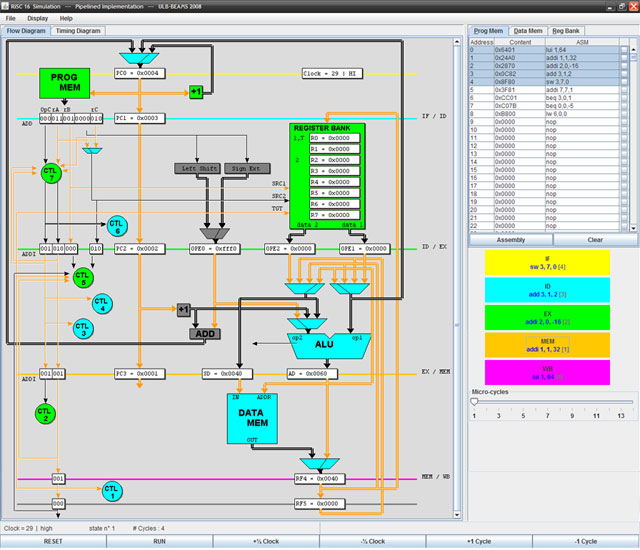
\includegraphics[width=15cm]{figures/100000000000028000000226ACEB2984.jpg}
	\end{center}
\caption{Pipelined RiSC-16 processor}
\label{fig:risc}
\end{figure}

The pipeline has 5 stages and instructions are split into:
\begin{enumerate}
\item \textbf{IF} (Instruction Fetch): instruction is read from program memory. \verb!PC! is also incremented.
\item \textbf{ID} (Instruction Decode): opcode is decoded and operands for ALU are read in the register bank
\item \textbf{EX} (EXecute): ALU processes the operation
\item \textbf{MEM} (MEMory): access to Data Memory
\item \textbf{WB} (Write-Back): result is written in destination register
\end{enumerate}


The interface presented in the simulator is designed in the same way that the sequential version to ease switching between the two implementations.

There are several zones in the simulator window:
\begin{itemize}
\item The execution zone has two tabs:
\begin{itemize}
\item The first one shows the steps of a cycle
\item The second one shows the cycle-instruction diagram (see Figure \vref{fig:pipe}). The number of cycles per instruction (CPI) is also shown.
\end{itemize}
%this gives the result:\\
\begin{figure}[h!]
	\begin{center}
		\begin{tabular}{r *{5}{C{1cm}}}
\toprule
  	Stage:			& 1	& 2 & 3 & 4 & 5 \\ 
 \midrule
\color{blue}lui 1, 64 \color{red}[0] 	& \cellcolor{yellow}IF& \cellcolor{cyan}ID & \cellcolor{green}EX &  \cellcolor{orange}MEM & \cellcolor{magenta}WB \\ 
\color{blue}addi 1, 1, 32 \color{red}[1] 	&  	& \cellcolor{yellow}IF & \cellcolor{cyan}ID &  \cellcolor{green}EX & \cellcolor{orange}MEM \\ 
\color{blue}addi 2, 0, -16 \color{red}[2] &   &   & \cellcolor{yellow}IF & \cellcolor{cyan}ID & \cellcolor{green} EX \\ 
\color{blue}add 3, 1, 2 \color{red}[3] 	&  	&   &   & \cellcolor{yellow}IF & \cellcolor{cyan}ID \\ 
\color{blue}sw 3, 7, 0 \color{red}[4] 	&   &   &   &   & \cellcolor{yellow}IF \\ 
\bottomrule
\end{tabular}
	\end{center}
\caption{Pipeline execution}
\label{fig:pipe}
\end{figure}

\item The memory zone on the right has 3 tabs to show and edit content of program memory, data memory and file register.
\item Another zone on the right details the content of the pipeline for each stage and the cursor shows the current step of the cycle.
\item The lower part groups the interaction possibilities: buttons provide reinitialisation (reset), execution (run), instruction execution and undo last clock-cycle capabilities. 
\item The central zone shows the blocks for this architecture.
\end{itemize}

Internal blocks of the processor have two particularities:
\begin{enumerate}
\item The control unit is split into several smaller units. Each one has a specific role either for a flawless execution or for managing pipeline hazards.
\item Between each stages, Pipeline registers were added to store states variables related to the current stage. Among these variables, we can find the opcode, address of registers, state of the \verb!PC!\dots 
\end{enumerate}
Thanks to these registers the pipeline can work as expected because they are the link between stages.
Only pipeline registers and control unit are synchronous. Other blocks are asynchronous.
The Figure \vref{fig:seq} shows the execution sequence of instructions.
\begin{figure}[h!]
\setlength{\tabcolsep}{3pt} %no extra space in cells to keep constant tabular width
\footnotesize
	\begin{center}
%		\includegraphics[width=15cm]{figures/-crop.pdf}
\begin{tabular}{r|*{2}{C{0.5cm}}|*{2}{C{0.8cm}}|cC{1.3cm}|C{0.8cm}c|c|c|c|C{1.5em}|C{0.5cm}C{0.5cm}}
\toprule
\textonehalf cycle & 1 & 2 & 3 & 4 & 5 & 6 & 7 & 8 & ~9 & 10 & 11 & 12 & 13 & 14 \\ 
 \midrule
\cellcolor{yellow}Fetch & \multicolumn{2}{|c|}{\cellcolor{yellow}+1,ROM} & \cellcolor{yellow}ROM  &   &   &   &   &   &   &   &   &   & \cellcolor{lightgray} & \cellcolor{lightgray} \\%
\cellcolor{cyan}Decode & \multicolumn{2}{|C{1.3cm}|}{\cellcolor{cyan}CTL7, \newline LS, SE, \newline RF(src1)} &  \cellcolor{cyan}RF (src1) &   & \multicolumn{2}{|C{1.3cm}|}{\cellcolor{cyan}CTL6} & \multicolumn{2}{|C{1.6cm}|}{\cellcolor{cyan}MUXs2,\linebreak MUXOPE0} & \multicolumn{3}{|c|}{\cellcolor{cyan}RF(src2)}&  & \cellcolor{lightgray} &\cellcolor{lightgray} \\ 
%
\cellcolor{green}Execute & \multicolumn{2}{|C{1.3cm}|}{\cellcolor{green}CTL5, (+1)} & \multicolumn{2}{|C{1.8cm}|}{\cellcolor{green}CTL4,\linebreak ADD,\linebreak MUXalu1, MUXalu2} &  \multicolumn{2}{|C{1.3cm}|}{\cellcolor{green}CTL3, MUXop2} & \multicolumn{2}{|c|}{\cellcolor{green}ALU} & \multicolumn{2}{|c|}{\cellcolor{green}CTL3} & \multicolumn{2}{|c|}{\cellcolor{green}MUXpc} &\cellcolor{lightgray} &\cellcolor{lightgray}  \\ 
%
\cellcolor{orange}Memory & \multicolumn{2}{|c|}{\cellcolor{orange}CTL2} & \multicolumn{2}{|c|}{\cellcolor{orange}RAM} & \multicolumn{1}{|C{1.3cm}|}{\cellcolor{orange}RAM, \linebreak CTL2} & \cellcolor{orange}CTL2 & \multicolumn{2}{|c|}{\cellcolor{orange}MUXrf4} &   &   &   &  & \cellcolor{lightgray} & \cellcolor{lightgray} \\ 
\cellcolor{magenta}Write Back &   &   & \multicolumn{2}{|c|}{\cellcolor{magenta}CTL1} & \multicolumn{3}{|c|}{\cellcolor{magenta}RF} &   &   &   &   & & \multicolumn{2}{c}{\multirow{-10}{1.2cm}{\cellcolor{lightgray}\centering Pipeline register update}} \\ 
\bottomrule
\end{tabular} 
	\end{center}
\caption{Instruction sequencing}
\label{fig:seq}
\end{figure}

The architecture performance can be measured using the cycles per instruction (CPI).
%
An ideal CPI for a pipeline should be 1 after each cycle, that means that an instruction ends at each cycle.
%
But actually, the pipeline is subject to hazards. In this RiSC16 architecture, only dependency conflicts (Data Hazards) and control problems (Control Hazards) can occur.

\subsection{Dependency hazards}
Dependency conflicts happens when an instruction needs a result from a previous instruction which is not completed yet. Only incidents of type ``Read After Write" can happen in the RiSC16.
To solve this problem, several possibilities exist:
\begin{itemize}
\item Data forwarding: a value is taken from a previous stage before its written in the register bank and is used as input to the ALU. Thanks to this mechanism, there is no penalty. Data forwarding is signalled by a message in the simulator.
\item When the \verb!LW! instruction is in stage EX and an instruction in ID stage uses an operand at the same address than the destination register for the \verb!LW! instruction, a Data hazard occurs. This hazard cannot be solved using Data forwarding, the only way to solve the issue is to stall the pipeline and so add a ``bubble". This will add a penalty of one cycle. This is signalled by a \textit{stall event} in the simulator.
\end{itemize}

\subsection{Control conflicts}
Control conflicts happens because of branch and call procedures. The address of the next instruction is computed in the execute stage an so, when a jump occurs, instructions loaded in the 2 previous stages are irrelevant and are discarded. This accident adds a penalty of 2 cycles and is named \textit{stomp event} in the simulator.

Various information messages are displayed when an accident occurs. They can be disabled using the ``Display > Alerts" menu.

\section{Manipulation}
\textit{Note: there is no assignment this week.}
\begin{Q}
Reuse the example of the first lab and draw the cycle-instruction diagram for the 25 first cycles. Compare the result with the simulation. Beware, accidents happen in simulation.
\end{Q}

\begin{Q}
What is the function of each control unit? Which are used during accidents solving?
\end{Q}

\begin{Q}
\label{Q:X}
Correct the program to suppress data hazards.
\end{Q}


\begin{Q}
Observe the CPI at the end of program execution and compare with the result of first lab.
\end{Q}

\begin{Q}
Find a way to compute the CPI using:
\begin{itemize}
\item pipeline ${depth}$ (here: 5)
\item instruction fully executed: ${instruction}$
\item number of stall events: ${stall}$
\item number of stomp events: ${stomp}$
\end{itemize}
\end{Q}

\begin{Q}
How would you modify the hardware to improve the design?
\end{Q}

\end{document}
